
\section{Questions, hypotheses and findings}

The questionnaire starts with recalling the European debt
crisis that began in 2010, and the \textit{Memoranda of Understanding}
that Greece, Spain, Portugal, Ireland and Cyprus signed with the European
Union, the European Central Bank and the International Monetary Fund that  
established financial aid combined with economic adjustment. We refer to
these contracts as \textit{aid\&reform} programs. 

We asked the respondents for each of the 19 EMU member whether
this was a program country, where a respondent could answer "yes",
"no", or "I don't know". The question has two purposes. First, it provides
information about the aggregate state of information. There are multiple
ways to aggregate the answers from 19 questions. %\footnote{%
%A very small number of experts found this question imprecisely stated. \emph{%
%We omit these replies the statistical analysis of this question?}} 
We
calculate a simple score:\ we count the number of program countries
correctly identified and deduct the number of wrong answers (both if a
respondent names a non-program country as program country or if the
respondent thinks that a program country did not sign a memorandum). Thus, the maximum score participants can obtain is 5, the minimum score -19. On
average, these numbers are

\begin{equation*}
\begin{tabular}{lll}
& Experts & Non-Experts \\ 
from borrower countries & $%
\begin{array}{c}
2.48 \\ 
(2.62)%
\end{array}%
$ & $%
\begin{array}{c}
1.10 \\ 
(2.74)%
\end{array}%
$ \\ 
from lender countries & $%
\begin{array}{c}
.78 \\ 
(3.50)%
\end{array}%
$ & $%
\begin{array}{c}
-.96 \\ 
(3.59)%
\end{array}%
$%
\end{tabular}%
\end{equation*}%
Experts were somewhat better informed than non-experts and participants from borrowers countries were somewhat better informed than participants from lender countries. The scores for experts from borrower and lender countries (2.48 and 0.78) are larger than the scores for non-experts from borrower and lender countries (1.10 and -0.96). The differences in the individual scores do, however, not turn out to be statistically significant.

We now turn to the questions that examine collective
self-serving memory biases. We ask whether country
origin matters for respondents' opinions about the \textit{reasons} for why lender countries wanted to engage in the credit relationship. 
\begin{figure}[h!]
\caption{Reasons of the lender countries for entering the rescue program}
    \begin{center}
    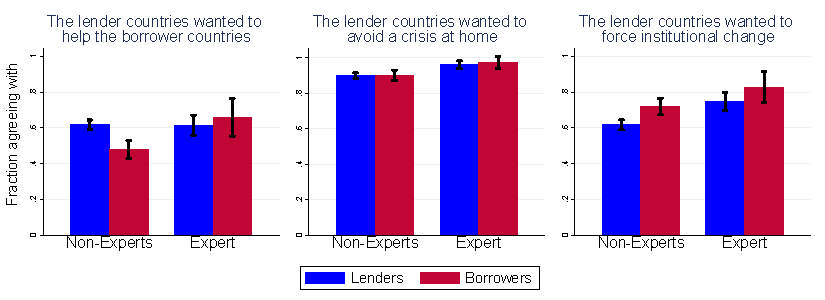
\includegraphics[scale=1.2]{graph2.pdf}
    \label{fig:Figure1}
    \end{center}
     \tiny
     \begin{tablenotes} 
    {The exact wording of the question is: In your opinion, what is the main reason why these countries entered these programmes 2a The lender countries wanted to help the borrower countries; 2b The lender countries wanted to help themselves to avoid a major crisis at home; 2c The lender countries wanted to force their desire for institutional change upon the borrower countries. Participants could choose the options strongly agree, slightly agree, slightly disagree and I don't know. We exclude all participants who answered with I don't know.\\
    The whiskers represent the 95 \% confidence intervals}
    \end{tablenotes}
\end{figure}

The nation-serving hypothesis is:\ respondents from borrower countries tend
to agree less frequently than respondents from lender countries 
that the lender countries wanted to help. They agree more that
the lender countries wanted to help themselves, and they agree more 
often that the lender countries wanted to force institutional change on the
crisis countries.\textit{\ }

The nation-serving hypothesis is not rejected based on our data (\autoref{fig:Figure1}). The share of non-experts from lender countries agreeing that lender countries wanted to help the borrower countries (62\%) is larger than the share of non-experts from borrower countries (48\%)
The difference in assessments between
non-experts from borrower and lender countries are large and statistically
significant at the 1 \% level for the aspect of reforms. There is also some disagreement in the expert sample. The differences, however, do not turn out to be statistically significant. \\
It is conceivable that
many non-expert respondents in the borrower countries were suspicious that
the lender countries had an institutional-reform agenda that goes beyond the
idea of helping each other. Participants from borrower and lender countries largely agree that lender countries wanted to avoid a crisis at home both in the expert and non-expert sample. The nation-serving bias manifests itself again in the non-expert sample in the question about the desire for institutional change among the lender countries. 62 \% of non-experts from lender countries agree with this statement compared to 72 \% among the lender countries. Again, we can observe differences in answers among the expert sample as well which are again not statistically significant. 
It is conceivable that experts, apart from simply being
better informed, often identify less with their own countries of origin and have 
a more cosmopolitan orientation. (At
least, this was the hypothesis that guided us to subject non-expert
nationals from the different countries to the same survey). Therefore, the
forces for developing a nation-bias might be less strong for experts than for non-experts. 

\begin{figure}
    \begin{center}
      \caption{Driving Force and Beneficiaries}
    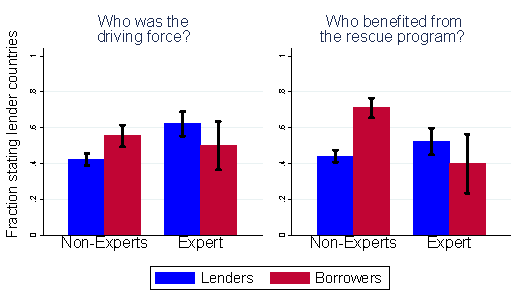
\includegraphics[scale=1.2]{graph3.pdf}
  
    \label{fig:figure2}
    \end{center}
    \tiny
    \begin{tablenotes} 
    {The exact wording of the questions is: 3. In formal terms, the borrower countries that signed a memorandum had to apply for support. But thinking about the true motivations and the political processes behind these events, which of the following three alternatives corresponds most closely to your perceptions. Answer options: The borrower countries wanted it, the lender countries were more reluctant; The lender countries wanted it, the borrower countries were more reluctant; Both wanted it equally; I don't know \\
   Question 4: Who do you think mainly benefited from the rescue program. Answer options: The borrower countries; The lender countries; Both groups of countries benefited equally; I don't know. We exclude all participants who answered with I don't know. \\
   The whiskers represent the 95 \% confidence intervals.}  
    \end{tablenotes}
\end{figure}
We
turn now to the next two questions.
Question 3 is similar to question 2 and asks about underlying motivations
and intentions. Question 4 asks about the beneficiaries of the aid\&reform
programs. The questions corroborate that the difference in nation-bias is a more systematic pattern (\autoref{fig:figure3}). Both questions show very similar patterns for non-expert
respondents, depending on whether they are from borrower countries or from
lender countries. The results suggest large and significant nation-biases. Non-experts
from borrower countries tend to see the lender countries as the main
motivators for these programs, in any case, more than respondents from the
borrower countries. This result corroborates the results on
self-serving memories from private informal lending as in \cite{dezso}, who report a tendency to assign the initiative\
for such contracts to the respective other side of the credit relationship. 

Non-experts from borrower and lending countries also differ in
their perceptions of who mainly benefited from the aid\&reform programs. The
bias tends to assign the benefits more to the counterparty group:\
respondents from borrower countries think more often than respondents from
lender countries that the lender countries are the major beneficiaries. These numbers
suggest that there is a nation-serving bias. 

The responses of experts do not seem to be prone to a country-group
bias. Whether an expert is originally from a borrower country or a lender
country does not affect their assessments about the
motivations driving the aid\&reform programs, nor their assessments about
who was the main beneficiary. \footnote{98 percent of experts also works in their country of origin }  Interestingly, there is a nation-disfavoring bias in the sample of experts. Experts from lender countries are 12 percentage points more likely to agree that lender countries were the driving force and the main beneficiaries of the rescue program. However, these differences do not turn out to be statistically significant.

We now turn to questions addressing how the groups of respondents
assess the implications of the aid\&reform programs for feelings among the
populations in the borrower and the lender
countries. The respondents' perceptions might be formed by direct
observations in the countries or media reports, but their views about the
reasons and motivations for the aid\&reform programs and their views about
who actually benefited from these programs should correlate with their
assessments, and might cause their beliefs about these feelings. 

We ask whether respondents think that the rescue experience might
have caused feelings of \textit{guilt}, feelings of \textit{being
exploited}, and/or feelings of \textit{inferiority}. The answers to these
questions, and possible differences for respondents from lender countries or
from borrower countries hardly report
nation-serving collective memory biases, but might rather be the outcomes of
such biases. Consider a citizen in the borrower country, say Greece. This
citizen may truthfully state what he or she believes what the
co-citizens in Greece feel. For instance, whether or not they feel guilt.
This feeling might, among other factors, be a result of a (potentially
nation-serving) view about how the crisis came about, and how Greece
addressed the crisis. If the views about reasons/motivations and the
distribution of benefits for the aid\&reform programs are self-serving, then
the Greek citizen might not see any reason for guilt:\ the crisis was just
bad luck, Greece was forced to take up more than the right amount of
(painful) reforms, and the benefits from these measures went elsewhere.
Hence, the Greek population might not see any reason to feel guilty.
Assessing the positions of respondents in the lender countries, these might
think that the crisis was caused by poor pre-crisis politics in Greece, that
Greece got a lot of assistance (see the previous questions) and resisted to
follow the Troika advice on necessary reforms for recovery. What does this
perception mean for beliefs about guilt? The respondent from the lender
country might think:\ if I were them, for what they have done, I would feel
guilty. The respondent might also have second-order beliefs.\ The respondents
might understand that the citizens in Greece perceived matters in a
nation-serving way and therefore will not feel guilty. While this modifies
possible expected outcomes, overall this reasoning points at a
borrower-country bias towards not agreeing that the citizens of these
countries feel guilty. 

NIKLAS: WOLLEN WIR DIE FN 6 rausnehmen?
\footnote{Our findings can also be interpreted in an alternative way.  Having a self-serving or nation-serving bias might make individuals oblivious to
the way policies are received in other countries. 
\cite{dezso} refer to this phenomenon as having a ``blind spot" regarding the other party's 
feelings and emotions. The hypothesis on the existence of such a ``blind spot" is confirmed in our findings.
Citizens from lender countries are more likely to agree that they felt guilty, exploited and/or inferior as a 
consequence of the rescue program. The largest difference between lender and borrower countries occurs with regards to feeling exploited.
78 percent  of citizens from borrower countries state that they felt exploited due to the rescue program while only 61 percent of lender countries
agree to this statement. 
}

%Similar reasons might let us suspect that the respondents from the lender
%countries are more inclined to think their population feels exploited, or
%feel inferior (in the sense of humiliated). Figure xxx shows the answers.
%First statistics negate the existence of a blind spot among borrowers about the feelings
%from citizens to lender countries. 

\begin{figure}
\begin{center}
    \caption{Emotions of the borrower countries}
    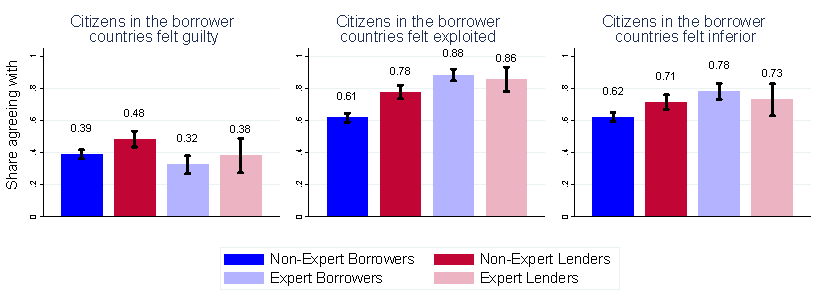
\includegraphics[scale=1.2]{graph5_1.pdf}
    \label{fig:figure3}
    \end{center}
    \tiny 
      \begin{tablenotes} 
      {The exact wording of the question was the following: Please give assessments of the following questions: 5a) The rescue experience made many citizens in the borrower countries feel guilty 
      5b) The rescue experience made many citizens in the borrower countries feel exploited 5c) The rescue experience mad many citizens in the borrower countries feel inferior
      Answer options: strongly agree, slightly agree, slightly disagree, strongly disagree, I don't know. We exclude all participants who answered with I don't know. \\
      The whiskers represent the 95 \% confidence intervals.}
      \end{tablenotes}
\end{figure}

We might expect that experts have a view on these questions that is hardly influenced by their countries of origin, such that we would not find much
difference in the responses of participants who originated in the borrower
countries and those of participants who originated in the lender countries (\autoref{fig:figure3}).


Similar questions assess the perceptions in the groups about the
feelings in the lender countries. In particular, we asked the participants whether they
agree on that the aid\&reform programs made the citizens in the
lender countries feel exploited and disappointed (\autoref{fig:figure4}). The non-experts in the lender
countries should be prepared to report their own feelings. However, the
perceptions about these lender-country feelings by the respondents from the
borrower countries might be distorted for several reasons. If they believe
that the lender countries are the true winners of these programs and that
this is how the citizens in these countries feel about it, they should agree
less to the ideas that citizens in lender countries feel exploited and
disappointed. If, however, they have second-order beliefs and can
successfully place themselves in the shoes of lender-country citizens, they
might understand that their beliefs about how the crisis came about and who
benefited from the programs are quite different, and they might correctly
assess their true feelings of being exploited and disappointed. Overall,
however, we might expect that the lender-country respondents agree more
frequently than the borrower-country respondents to the possibly negative
feelings in lender countries:

\begin{figure}[h!]
  \begin{center}
       \caption{Emotions of the lender countries}
    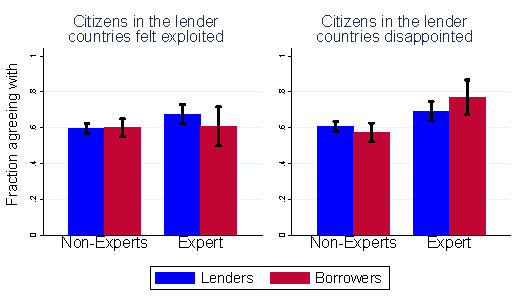
\includegraphics[scale=1.2]{graph5_2.pdf}
 
    \label{fig:figure4}
    \end{center}
    \tiny
    \begin{tablenotes}
     {The exact wording of the question is: 5d) The rescue experience made many citizens in the lender countries feel exploited 5e) The rescue experience made many citizens in the lender countries feel disappointed
    Answer options: strongly agree, slightly agree, slightly disagree, strongly disagree, I don't know. We exclude all participants who answered with I don't know. \\
    The whiskers represent the 95 \% confidence intervals}
    \end{tablenotes}
\end{figure}

We compare non-experts and experts. The results do not suggest that respondents from borrower countries have different views than respondents from lender countries. The findings indicate that the respondents
in both groups of countries believe that the \textit{aid\&reform programs} triggered
bad feelings in both groups of countries. A large share of the respondents
thinks that citizens in borrower countries feel guilty, exploited, and
inferior, and a large share of respondents also thinks that citizens in
lender countries feel disappointed and exploited as well. 

We have also asked whether the \texti{aid\&reform programs} strengthened friendship between the citizens in the Eurozone. The theory of groups and conflicts shows that, when groups jointly master a major task which none of them could have mastered in isolation, they overcome negative attitudes and mutual spite between groups. The European debt crisis had the potential to be 
such a task. It might have strengthened friendship between these groups.
However, if both groups have nation-serving diverging biases about what
motivated the crisis and the solution method adopted, and about the
distribution of the benefits and costs of the method adopted, then we might
expect that a large fraction of the respondents of both groups think that
these programs did not strengthen friendship ties. 
\begin{figure}
\begin{center}
\caption{Impact on friendships}
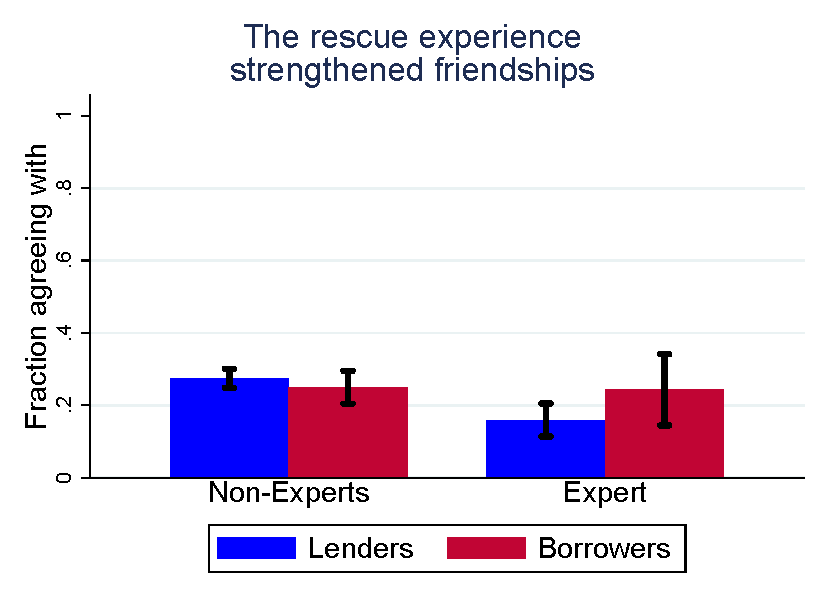
\includegraphics[scale=0.5]{graph5_3.pdf}
\label{fig:figure5}
\end{center}
\tiny 
\begin{tablenotes}
  {The exact wording of the question is the following: 5f) The rescue experience strengthened friendships
   Answer options: strongly agree, slightly agree, slightly disagree, strongly disagree, I don't know. We exclude all participants who answered with I don't know. \\
     The whiskers represent the 95 \% confidence intervals}
    \end{tablenotes}
\end{figure}

The majority of participants from the expert and non-expert sample disagrees that 
the rescue package strengthened friendships (\autoref{fig:figure5}).\footnote{Due to a survey error this question was displayed as "The rescue experience strengthened friendship ties between borrower". The fraction of experts who answered this question with "I don't know" lies around 20 percent. This is very much in line with the frequency of "I don't know" responses throughout the survey. Hence, it seems plausible that participants correctly understood the question. } This holds for participants from 
both the expert and the non-expert sample. This finding is also in line with the nation-serving biases
we find throughout the survey. In light of the absence of such a bias among the expert sample 
it seems interesting that the level of agreement in this sample is also quite low. 
This might suggest that although experts might not have and be aware of a nation-serving bias
among citizens from the lender countries they are indeed aware of the consequences of such 
a nation-serving bias. 
\\

The answers to the individual questions are likely to
be interdependent. For example, individuals in lender countries who
think that the borrower countries pushed for the aid\&reform programs
(questions 2 and 3) may also think that these are the main beneficiaries
(question 3), and therefore think that the lender countries feel exploited
and disappointed. The direction of causality for respondents from the lender
countries would be%
\begin{equation*}
\begin{array}{ccccc}
\begin{array}{c}
\text{borrower countries} \\ 
\text{pushed for aid\&reform}%
\end{array}
& \rightarrow  & 
\begin{array}{c}
\text{borrower countries} \\ 
\text{are the main} \\ 
\text{beneficiaries of} \\ 
\text{aid\&reform}%
\end{array}
& \rightarrow  & 
\begin{array}{c}
\text{lender countries} \\ 
\text{feel exploited} \\ 
\text{and disappointed.}%
\end{array}%
\end{array}%
\end{equation*}


We evaluate this chain of causality empirically: 
\begin{table}[h!]
    \centering
    \begin{tabular}{c|c}
         &  \\
         & 
    \end{tabular}
    \caption{Empirical Assessment of chain of causation }
    \label{tab:my_label}
\end{table}

\begin{table}[h!]
\begin{center}

\begin{tabular}{l*{1}{cccc}}
\hline\hline
                    &\multicolumn{4}{c}{}                               \\
 The lender countries were the driving force                   &   4 & 5.1 & 5.2 &  5.3 \\
\hline
Answers of people disagreeing                &        0.32&        0.40&        0.63&        0.65\\
Answers of people agreeing                &        0.70&        0.40&        0.78&        0.72\\
\hline
Total               &        0.51&        0.40&        0.70&        0.68\\
\hline\hline
\end{tabular}
\end{center}
\begin{tablenotes}
\item \tiny Conditional on participants agreeing or disagreeing with the lender countries being the driving force for the aid & reform program we present the likelihood to state lender countries as an answer to question 4 (Who mainly benefited from the reform), Question 5.1 (The rescue experience made citizens in the borrower countries feel exploited); Question 5.2 (The rescue experience made many citizens in the borrower countries feel exploited) Question 5.3 (The rescue experience made many citizens in the borrower countries feel inferior)
\end{tablenotes}
\end{table}

\begin{table}[h!]
   \begin{center}
\begin{tabular}{l*{1}{ccc}}
\hline\hline
                    &\multicolumn{3}{c}{}                  \\
Lender countries were main beneficiaries                    &  5.1 &  5.2 &  5.3 \\
\hline
Answers of people disagreeing           &        0.35&        0.58&        0.58\\
Answers of people agreeing                   &        0.45&        0.81&        0.74\\
\hline
Total               &        0.40&        0.70&        0.66\\
\hline\hline
\end{tabular}
\end{center} 
\begin{tablenotes}
\item \tiny
Conditional on participants stating that lender countries benefiting from the aid & reform program we present the likelihood to agree with Question 5.1 (The rescue experience made citizens in the borrower countries feel exploited); Question 5.2 (The rescue experience made many citizens in the borrower countries feel exploited) Question 5.3 (The rescue experience made many citizens in the borrower countries feel inferior)
\end{tablenotes}
\end{table}
The results suggest that participants who agree with the statement that the borrower (lender) countries were the driving force behind the reform are also more likely to agree that the borrower (lender) countries were the main beneficiaries of the aid& reform package. The assessment of which party was the driving force does not influence participants opinions on the feelings that were evoked among borrower or lender countries. However, participants who agree with the statement that the lender countries were the main beneficiaries from the rescue program also show a higher likelihood to agree that the borrower countries felt guilty/ exploited or inferior due to the rescue program. For participants who agree that the 
respondents from the borrower countries who think that the lender countries
pushed for the aid\&reform programs, wanted to impose institutional reforms
on them are probably the same who think that the lender countries are the
main beneficiaries, and also the same ones who think that the borrower
countries have been exploited and would not feel guilt, but feel humiliated
("inferiority"?). The direction of causality is%
\begin{equation*}
\begin{array}{ccccc}
\begin{array}{c}
\text{lender countries} \\ 
\text{pushed for aid\&reform} \\ 
\text{and wanted to impose} \\ 
\text{structural reforms}%
\end{array}
& \rightarrow  & 
\begin{array}{c}
\text{lender countries} \\ 
\text{are the main} \\ 
\text{beneficiaries of} \\ 
\text{aid\&reform}%
\end{array}
& \rightarrow  & 
\begin{array}{c}
\text{borrower countries} \\ 
\text{feel exploited}%
\end{array}%
\end{array}%
\end{equation*}
\begin{table}
  \begin{center}
\begin{tabular}{l*{1}{ccc}}
\hline\hline
                    &\multicolumn{3}{c}{}                  \\
                    & 4& 5.4 &  5.5 \\
\hline
0                   &        0.24&        0.59&        0.61\\
1                   &        0.47&        0.65&        0.63\\
Total               &        0.33&        0.61&        0.62\\
\hline\hline
\end{tabular}
\end{center}
\begin{tablenotes}
\item \tiny Conditional on participants agreeing or disagreeing with the borrower countries being the driving force for the aid & reform program we present the likelihood to state borrower countries for question 4 (Who was the main beneficiary from the rescue program?), or agree with question 5.4 (The rescue experience made citizens in the lender countries feel exploited); Question 5.5 (The rescue experience made many citizens in the lender countries feel disappointed)
\end{tablenotes}
\end{table}

\begin{table} 
  \begin{center}
\begin{tabular}{l*{1}{cc}}
\hline\hline
                    &\multicolumn{2}{c}{}     \\
                    &  5.4  5.5 \\
\hline
0                   &        0.59&        0.60\\
1                   &        0.65&        0.65\\
Total               &        0.61&        0.62\\
\hline\hline
\end{tabular}
\end{center} 
\begin{tablenotes}
\item \tiny Conditional on participants stating that borrower countries did or did not benefit from the aid & reform program we present the likelihood to agree with Question 5.4 (The rescue experience made citizens in the lender countries feel exploited); Question 5.5 (The rescue experience made many citizens in the lender countries feel disappointed)
\end{tablenotes}
\end{table}
\\
